%
% Documentation of the planar geometry algorithms used in the
% Mini Jam project du on October 31st, 2024.
% The game is called "Ardymo", a combination of "Arduino" and "Waymo"
%
% Compute the intersections of a straight line with an ellipse and
% a rectangle.
%
\documentclass[11pt]{article}
%
% Packages
%
\usepackage{graphicx}
\usepackage{array}
\usepackage{amsmath,bm}
\usepackage{color}
% \usepackage{paralist}
%
% Dimensions
% \setlength{\textwidth}{5.5in}
% \setlength{\textheight}{8.4in}
% \setlength{\hoffset}{-0.25in}
% \setlength{\topmargin}{0pt}
\setlength{\parindent}{0pt}
\setlength{\parskip}{0.5\baselineskip}
%
% Definitions
% Mathematical symbols
\newcommand{\Rb}{{\mathbf{R}}}
\newcommand{\diota}{d_\iota}
\newcommand{\xiota}{x_\iota}
\newcommand{\xsigma}{x_\sigma}
\newcommand{\yiota}{y_\iota}
\newcommand{\ysigma}{y_\sigma}
\newcommand{\bhat}{{\hat{b}}}
\newcommand{\xhat}{{\hat{x}}}
\newcommand{\yhat}{{\hat{y}}}
\newcommand{\bfx}{\mathbf{x}}
% Labels and text
\newcommand{\eqn}[1]{(\ref{#1})}
\newcommand{\figref}[1]{Fig.~\eqref{#1}}
\newcommand{\TODO}{{\bf TODO}}
% For graphics alignment:
\newcommand{\HR}{\rule{1em}{0.4pt}}
\newcommand{\bluefbox}[1]{\textcolor{blue}{%
        \setlength\fboxsep{0pt}\fbox{\textcolor{black}{#1}}}}

\begin{document}
%
%
\title{Planar Geometry}
\author{Aurel Wisse}
\maketitle
%
%
\begin{abstract}
Documentation of the planar geometry algorithms used in the
Mini Jam project due on October 31st, 2024. We present the algorithms used to
compute the intersection of straight lines (sensor ray for identification
of obstacles) with circles, rectangles and line segments.
\end{abstract}

%
\section{Straight Line}
\label{sec-straight-line}

\subsection{Unbound}
\label{sec:unbound}
We develop the representation of a straight line going through
coordinates $(x_0, y_0)$ and $(x_1, y_1)$. Let us determine the points $(x,
y)$ on the line.

We have two special cases:
\begin{eqnarray}
    (x, y) &=& (x_0, y)\quad\forall y\in\Rb\quad \text{ if } x_1 = x_0
    \label{eq-line-xx0} \\
    (x, y) &=& (x, y_0)\quad\forall x\in\Rb\quad \text{ if } y_1 = y_0
    \label{eq-line-yy0}
\end{eqnarray}

For the general case, $x_0 \neq x_1 \land y_0 \neq y_1$, we have
\begin{eqnarray}
    y &=& ax+b,\quad \forall x\in\Rb\quad \text{where}\label{eq-line-general}\\
    a &=& \frac{y_0 - y_1}{x_0 - x_1}, \notag \\
    b &=& \frac{x_0 y_1 - y_0 x_1}{x_0 - x_1} \notag
\end{eqnarray}

\subsection{Line Segment}
\label{sec-line-segment}
A line segment is the compact version of a straight line. It is of finite
length. For the special case $x_0 = x_1$ the points $(x, y)$ on the line
segment $[(x_0, y_0):(x_0, y_1)]$ between $(x_0, y_0)$ and $(x_0, y_1)$ are
given by
\begin{equation}
    (x, y) = (x_0, y)\quad y\in [y_0, y_1]\label{eq-seg-x1x0}
\end{equation}

For the special case $y = b$ the points $(x, y)$ on the line segment
$[(x_0, b):(x_1, b)]$ are given by
\begin{equation}
    (x, y) = (x, b)\quad x\in [x_0, x_1]\label{eq-seg-yb}
\end{equation}

For the general case given by \eqn{eq-line-general}, the points $(x, y)$ on
the line segment $[(x_0, y_0):(x_1, y_1)]$ are given by
\begin{equation}
    (x, y) = (x, ax + b)\quad x\in [x_0, x_1]\label{eq-seg-general}
\end{equation}
where $a\neq 0$.

\section{Polygons}
\label{sec-polygons}

We are concerned with a general polygon in the two-dimensional plane. A polygon
with $n$ sides is well defined by $n$ line segments and $n$ points $(x_0,
y_0),\ldots,(x_{n-1}, y_{n-1})$. The $n$ sides are defined by the line segments
\begin{equation}
    \left\{[(x_i, y_i):(x_{i+1}, y_{i+1})], i=0,\ldots,n-2\right\}\\
\cup\left\{[(x_{n-1}, y_{n-1}):(x_{0}, y_{0})]\right\}
\end{equation}

\section{Rectangle}
\label{sec-rectangle}
While general polygons are useful as obstacles, they lack the direction
information we need for the vehicle.  Hence we define a rectangle with five
parameters by starting with a rectangle of which the sides are parallel to
the x-axis and the y-axis, given by the four parameters
\begin{enumerate}
    \item $(x_0, y_0)$ the center of the left side of the rectangle.
    \item $w$ the width (x-direction) of the rectangle.
    \item $h$ the height (y-direction) of the rectangle.
\end{enumerate}
The fifth parameter $\alpha$ represents the clockwise rotation of the 
rectangle around the point $\left(x_0, y_0\right)$. The parameters are 
illustrated in \figref{fig-rectangle}.

\begin{figure}
    \centering
    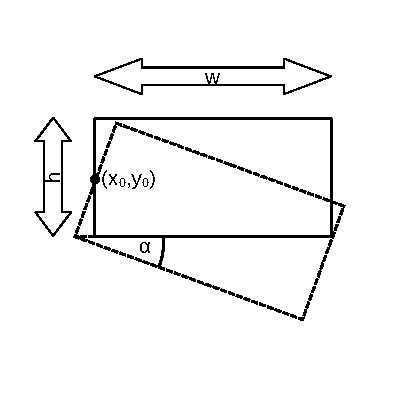
\includegraphics[trim=10 40 10 20]{rectangle.pdf}
    \caption{Rotated Rectangle}\label{fig-rectangle}
\end{figure}

\section{Circle}
\label{sec-circle}

The standard implicit equation for a circle of radius $r$  centered at the
point $(x_0, y_0)$ is
\begin{equation}
    (x - x_0)^2 + (y - y_0)^2 = r^2\label{eq-circle}
\end{equation}

\TODO: We might generalize to an ellipsis later if this adds something
interesting to the gameplay:
\begin{equation}
    \frac{(x-x_0)^2}{a^2} + \frac{(y-y_0)^2}{b^2} = 1
\end{equation}

\section{Intersection and Distance}
\label{sec-intersection-distance}

The general form of the distance $\diota$ between the origin of the sensor ray
$\bfx_\sigma=(\xsigma,\ysigma)$ and the point of intersection
$\bfx_\iota=(\xiota,\yiota)$ is given by Pythagoras' Theorem:
\begin{equation}
    \diota = \sqrt{(\xiota-\xsigma)^2 + (\yiota-\ysigma)^2}
\end{equation}

\subsection{Line Segment}
\label{sec-intersection-line-segment}

\subsubsection*{Intersection}
We must consider the intersections of all three possibilities of sensor rays
$(x, y) =(x_0, y)$ \eqref{eq-line-xx0}, $(x, y)=(x, b)$ \eqref{eq-line-yy0} 
and $(x, y) = (x, ax+b)$
\eqref{eq-line-general} with all three possibilities of line segments
$x_{s0}=x_{s1}$ \eqref{eq-seg-x1x0}, $y_{s0}=y_{s1}$ \eqref{eq-seg-yb} and
$y=a_{s}x+b_{s}$ \eqref{eq-seg-general}, where $(x_{s0}, x_{s1})$ are the
limits of the $x$-parameter, $(y_{s0}, y_{s1})$ the limits of the
$y$-parameter and $(a_{s}, b_{s}),\,a_{s}\neq 0$ the parameters of the general case
\eqref{eq-seg-general}.

We present the conditions for intersections of the sensor ray (first column)
with the line segments (first row) in
table~\eqref{tab-condition-intersection-seg}.
% Definitions: Math mode columns
\newcolumntype{C}{>{$\scriptstyle}c<{$}}
\newcolumntype{L}{>{$\scriptstyle}l<{$}}
% The table
\begin{table}
    \centering
    \begin{tabular}{L|CCC}
    \text{Sensor}& x_{s1}=x_{s0} & y_{s1}=y_{s0} & a_{s}x + b_{s} \\ \hline
    x=x_0 & x_0=x_{s0} & \multicolumn{2}{C}{x_{s0}\leq x_0\leq x_{s1}} \\
    y=b & y_{s0}\leq b\leq y_{s1} & b=y_{s0} &
    x_{s0}\leq \frac{b - b_s}{a_s}\leq x_{s1} \\
    ax+b & y_{s0}\leq ax_{s0}+b\leq y_{s1} &
    x_{s0}\leq \frac{y_{s0}-b}{a}\leq x_{s1} &
    \left\{\begin{tabular}{C}a=a_s\,\land\,b=bs\\ \text{or}\\
            x_{s0}\leq \frac{b_s-b}{a_s-a}\leq x_{s1}
        \end{tabular}\right\}
    \end{tabular}
    \caption{Conditions for intersections with line
    segments}\label{tab-condition-intersection-seg}
\end{table}

\subsubsection*{Distance}

Let ${\bfx}_\sigma=(x_\sigma, y_\sigma)$ be the origin of the sensor ray. We 
want to compute the distance between $\bfx$ and the point of intersection with
the line segment. In certain cases, there is more than one point of
intersection and we must choose the nearest. In Table~\eqref{tab-distance-seg}.

\subsection{Rectangle}
\label{sec-intersection-rectangle}

A rectangle is given by the parameters $(x_0, y_0, w, h, \alpha)$
(Section~\ref{sec-rectangle}). The rectangle is defined at the origin with
width $w$ and height $h$. The upper left corner of the rectangle at the
origin is at the point $\left(-\frac{h}{2},0\right)$.
The points of the rectangle are rotated clockwise around the origin by 
$\alpha$ and translated by adding the vector
$(x_0, y_0)$.

There are two ways to determine the intersection of the sensor ray with the
rectangle.
\begin{enumerate}
    \item Transform the rectangle into four line segments and
        proceed with the algorithm in
        section~(\ref{sec-intersection-line-segment}) for each segment.
    \item Rotate and translate the sensor ray by the inverse transformation of
        the rectangle: Translate by $(-x_0, -y_0)$ and rotate by $\-alpha$.
\end{enumerate}
We are using the second approach.

Let $(x, y)$ be a point on the sensor ray. Let $(\xhat, \yhat)$ the
corresponding transformed point, given by
\begin{eqnarray}
    \xhat &=& (x - x_0) \cos(\alpha) + (y - y_0) \sin(\alpha) \\
    \yhat &=& (x_0 - x) \sin(\alpha) + (y - y_0) \cos(\alpha)
\end{eqnarray}

\subsection{Circle}
\label{sec-intersection-circle}
For the sensor ray, we must consider the three cases $(x,y)=(x_0,y)\,\forall y$
\eqref{eq-line-xx0}, $(x,y)=(x,y_0)\,\forall x$ \eqref{eq-line-yy0} and $y=ax+b$
\eqref{eq-line-general}.

Let $(x_c, y_c)$ be the center of the circle.

For the case $(x,y)=(x_0, y)$, the intersection with the circle
$(x-x_c)^2+(y-y_c)^2=r^2$ is given by
\begin{equation}
    y = y_c \pm\sqrt{r^2 - (x_0-x_c)^2}.
\end{equation}
If $r^2 < (x_0-x_c)^2$, there is no intersection with the circle.

For the case $(x,y)=(x, y_0)$, the intersection with the circle
$(x-x_c)^2+(y-y_c)^2=r^2$ is given by
\begin{equation}
    x = x_c \pm\sqrt{r^2 - (y_0-y_c)^2}.
\end{equation}
If $r^2 < (y_0-y_c)^2$, there is no intersection with the circle.

For the general case, the intersection of a
straight line $y=ax+b$ with a circle $(x-x_c)^2+(y-y_c)^2=r^2$ is given by
\begin{equation}
    (x-x_c)^2 + (ax+b - y_c)^2 = r^2
\end{equation}
In order to simplify calculations, we translate the origin to $(x_c, y_c)$. Let
\begin{equation}
    \xhat = x-x_c,\quad \yhat = y-y_c,\quad \bhat = ax_c + b - y_c.
\end{equation}
The intersection of the straight line $\yhat = a\xhat + \bhat$ with the circle
$\xhat^2 + \yhat^2 = r^2$ is given by
\begin{equation}
    \xhat^2 + (a\xhat + \bhat)^2 = r^2 \label{eq-intersection-circle}
\end{equation}
The solutions $\xhat$ to \eqref{eq-intersection-circle} are given by
\begin{equation}
    \xhat = -\frac{a\bhat}{1+a^2}\pm
        \sqrt{\frac{1}{1+a^2}\left(r^2-\bhat+\frac{a^2 \bhat^2}{1+a^2}\right)}
\end{equation}
From this, we see that if
\begin{equation}
    r^2-\bhat+\frac{a^2 b^2}{1+a^2} < 0,
\end{equation}
there is no intersection of the line and the circle.

\section{Representation}
\label{sec-representation}
In this section we describe how circles, sensor rays and line segments will be
represented in code. There is no particular polygon object given that a
polygon is just a collection of line segments.

\subsection{Unbound Straight Line}


Parameters $(a, b, X, z_0, z_1)$.
The parameters $z_0, z_1$ are set to zero for an unbound line. They define
the endpoints of a line segment.

\begin{enumerate}
    \item For an unbound straight horizontal line, $a=X=0, y=b$.
    \item For an unbound straight vertical line, $a=b=0, x=X$.
    \item For an unbound general line, $X=0$.
\end{enumerate}

\subsection{Line Segment}
\label{sec-representation-line-segment}

Parameters $(a, b, X, z_0, z_1)$.

Covers all cases. We must define a transformation of the points $(x_0, y_0)$
and $(x_1, y_1)$  into a general straight line with inequalities:
\begin{equation}
    (a, b, X, z_0, z_1) =
    \begin{cases}
        (0, y_0, 0, x_0, x_1)  &
        \text{if $y_1 = y_0\land x_0 < x_1$}\\
        (0, 0, x_0, y_0, y_1) &
        \text{if $x_1 = x_0\land  y_0 < y_1 $}\\
        \left(\frac{y_0 - y_1}{x_0-x_1},
            \frac{x_0 y_1 - x_1 y_0}{x_0 - x_1}, 0, x_0, x_1\right) &
            \text{if $x_0< x_1\,\land\,y_0< y_1$}
    \end{cases}
\end{equation}

\subsection{Rectangle}

A rectangle is given by the parameters $(x_0, y_0, w, h, \alpha)$
(Section~\ref{sec-rectangle}).


\subsection*{Circle}

Parameters $x_0, y_0, r$.

\section{Game Objects}
\label{sec-game-objects}
There are four types of objects in the game.
\begin{enumerate}
    \item The game surface. A rectangle with $(0,0)$ in the upper left corner.
        It is defined by two values $x_G > 0, y_G>0$ respectively on the x-axis
        and the y-axis.
    \item The {\sl vehicle} which is a rectangle with a direction $\alpha$
    \item The target which is a single point $T = (x_T, y_T)$ on the game
        surface.
    \item The obstacles. A collection of line segments and circles.
\end{enumerate}

\section{The Game}
\label{sec-the-game}
\begin{itemize}
    \item There are two players in the game, one on each Arduboy.
    \item The objective of the game is to reach the target first without
        running into an obstacle.
    \item Running into an obstacle requires a repair of the vehicle and leads
        to a 30 second suspension.
    \item Colliding with the other players car from the side or behind places
        the player at the start with a 30 second suspension.
    \item A frontal collision of both players ends the game without a winner.
\end{itemize}

\subsection{User Interface}
\label{sec-user-interface}
The main screen Figure \figref{fig-main-screen}.
\begin{figure}
    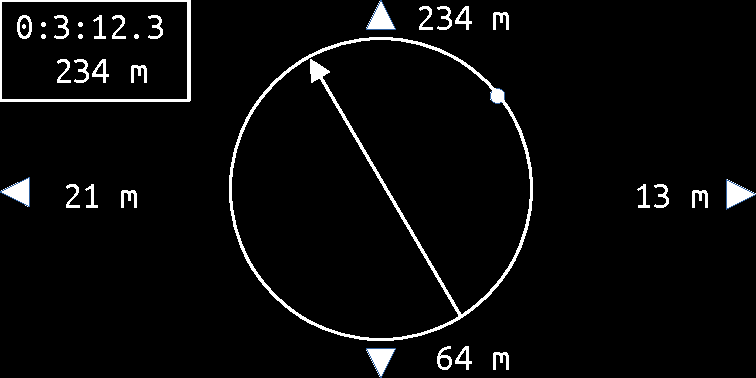
\includegraphics[width=\textwidth]{screen.pdf}
\caption{Mockup of the main game screen}\label{fig-main-screen}
\end{figure}
\begin{itemize}
    \item The numbers next to the four triangles, top, left right and botton
        show the distance to the nearest object (obstacle or target).
    \item The arrow shows the direction of the vehicle.
    \item The dot on the circle shows in which direction the target is
        located.
    \item The elapsed game time is the number at the top left in the white
        rectangle.
    \item The distance to the target is the number below the elapsed time.
\end{itemize}

\subsection{Game Map}
\label{sec-game-map}
The game map is a rectangle given by two values $x_M, y_M > 0$. The resulting
rectangle is defined by the four points
\begin{equation*}
    \{(0,0), (x_M, 0), (0, y_M), (x_M, y_M)\}
\end{equation*}
The map is filled with two vehicles, one for each player, a target and
obstacles which are a collection of line segments and circles.

Given that the map can be quite big, no bitmap representation of the game map
is displayed on the Arduboy. However, the map can be converted to a bitmap
with a suitable drawing program. Ultimately, a small program for conversion
into an SVG file can be written.

\subsection{Controls}
\label{sec-controls}

\begin{tabular}{>{\sffamily\bfseries}ll}
    Up Button & Accelerate forward $1m/s^2$. \\
    Down Button & Accelerate backwards (also "braking").\\
    Left Button & Turn left $\alpha$ degrees.\\
    Right Button & Turn right $\alpha$ degrees.\\
    A Button & TBD.\\
    B Button & Show menu.\\
\end{tabular}

\subsection{Vehicle Movement}
\label{sec-vehicle-movement}

The vehicle is defined as a rectangle given by four points. Two points at the
front of the vehicle and two points at the rear of the vehicle. These points
define four line segments.

Turning the vehicle with the left or right button rotates the four buttons
around the midpoint of the two points at the rear of the vehicle, as
illustrated in \figref{fig-vehicle-rotate}.
\begin{figure}
    \centering
    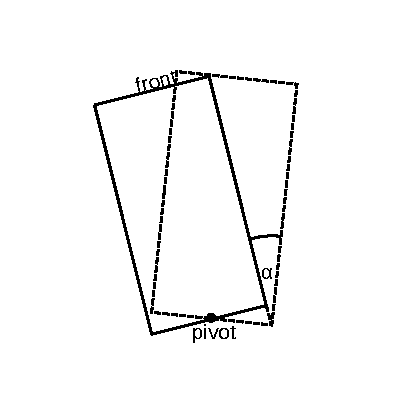
\includegraphics[trim=0 30 0 30]{vehicle-turn.pdf}
    \caption{Vehicle Turn}\label{fig-vehicle-rotate}
\end{figure}
The vehicles' forward movement is in the direction of the front of the vehicle
parallel to the sides of the vehicle.
The vehicles' backward movement is in the direction of the rear of the vehicle
parallel to the sides of the vehicle.

\subsection{Target and Obstacles}
\label{sec-obstacles}

The obstacles are line segments and circles. The target is a circle. The
vehicle is a rectangle. The limits of the game map are obstacles.

\pagebreak
\section{Scanning}
\label{sec-scanning}
In each frame, the vehicle scans for obstacles in the following way.

The straight lines prolonging the sides of the vehicle are checked for
intersections with all obstacles in the list. The distance to the closest
obstacle is displayed on the user interface.

The straight line perpendicular to the vehicle and running through the center
of the vehicle is checked for intersections with all obstacles in the list.
The distance to the closest obstacle is displayed on the user interface
\figref{fig-scanning}.

\begin{figure}
    \centering
    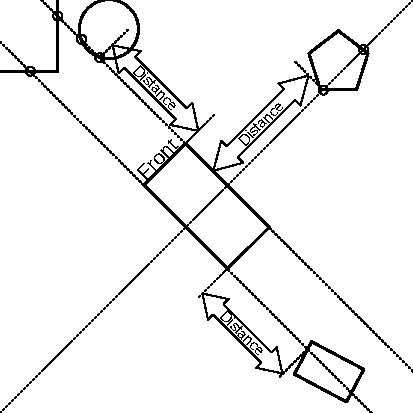
\includegraphics{scanning.pdf}
    \caption{Scanning and Distance}\label{fig-scanning}
\end{figure}

\end{document}
